\documentclass[journal=dce]{CUP-JNL-DTM}%

\usepackage{graphicx}
\usepackage{amsmath,amssymb,amsfonts}
\usepackage{booktabs}
\usepackage[numbers]{natbib}
\usepackage[T1]{fontenc}
\usepackage{lmodern}
\usepackage{textcomp}
\usepackage[colorlinks,allcolors=blue]{hyperref}

\jpub{CAMBRIDGE UNIVERSITY PRESS}
\jname{DATA-CENTRIC ENGINEERING}
\articletype{RESEARCH ARTICLE}
\jyear{2026}
\jvol{0}
\jissue{0}
\eissn{2632-6736}
% \jdoi intentionally omitted: no DOI has been assigned to this manuscript yet.

\begin{document}

\begin{Frontmatter}

\title[Cross-Domain Audit Protocol Reliability]{When Does a Cross-Domain Audit Protocol Actually Detect Universality? A Synthetic-Data Study of Scaling-Law Discovery Under Domain Confounding}

\author[1]{Jes\'us Gil Ruiz}
\author[2]{Roberto A. Pava-D\'iaz}
\author[2]{Carlos Enrique Montenegro Mar\'in}

\authormark{Gil Ruiz et al.}

\address[1]{\orgdiv{Science and Aerospace Department}, \orgname{Universidad Europea de Madrid}, \orgaddress{\city{Villaviciosa de Od\'on}, \country{Spain}}. \email{jesus.gil@universidadeuropea.es}}
\address[2]{\orgdiv{Faculty of Engineering}, \orgname{Universidad Distrital Francisco Jos\'e de Caldas}, \orgaddress{\city{Bogot\'a}, \country{Colombia}}}

\keywords{domain generalization, scaling-law discovery, leave-one-group-out cross-validation, bootstrap, synthetic benchmarking, model misspecification}

\abstract{Leave-one-group-out (here, leave-one-facility-out, LOFO) cross-validation with bootstrap resampling audits whether a data-driven scaling law generalizes across experimental sources or is an artifact of a single facility. Two companion manuscripts \citep{gilruiz2026paper1,gilruiz2026paper2} applied this protocol to a real 114-point windage (rotor-stator disc friction) dataset spanning four facilities and found that a good in-sample fit collapses under LOFO, and that classical and modern machine-learning models alike fail to recover a generalizing model. That negative result raises a question a single small dataset cannot answer: is the audit protocol itself reliable at that scale? We answer this with a synthetic study under known ground truth and four confounding mechanisms, adding real bootstrap resampling to match the companion manuscripts' methodology. The conventional LOFO R\textsuperscript{2}$>0$ declaration rule is reliable against parameter drift and heavy-tailed noise ($\sim$80\% correct verdicts when confounded), but has a severe, quantified blind spot: only 9.4\% of nonlinear-misspecified and 42.7\% of clustered (partially universal) scenarios are correctly flagged as non-generalizing, and detection does not improve with more facilities -- for nonlinear misspecification it gets worse (35.9\% at $K$=2--3 down to 0.7\% at $K$=16--20). A facility-label permutation test ($n_{\text{perm}}$=99, $\alpha$=0.05) computed from the same fits, at no extra data-collection cost, is a substantially more reliable replacement: 96.5\% vs.\ 90.1\% overall accuracy on the first pass, at the cost of lowering accuracy on truly universal scenarios from 100\% to $\sim$94--95\%. On the ambiguous confounded-only cases where the threshold rule degrades with $K$ (77--96\%), the permutation rule holds at 100\% for $K\geq4$. Its validity, however, is conditional on an assumption we make explicit and then test in a third pass of 6,000 scenarios: the permutation null requires facilities to share covariate support. As their operating windows separate, the naive permutation test becomes anti-conservative, with false alarms rising from 5.9\% at near-complete overlap to 17.2\% at near-disjoint support -- against a nominal 5\% -- while the threshold rule never false-alarms anywhere in the sweep. Permuting labels only within covariate strata restores calibration (4.6--6.2\% throughout) at essentially no cost in power ($\geq$97.7\%), and is the rule we ultimately recommend; only under near-total separation (overlap $<$0.02) does it also degrade, a regime where facility identity is nearly a deterministic function of the covariates and no label-permutation scheme can separate a different law from a different design. Because this choice depends on a quantity practitioners can measure, we report the corresponding support-overlap statistic for the companion corpus (mean pairwise overlap 0.32, with its largest facility almost disjoint from the other three), which places that case in the regime where the naive test would run at roughly 2.5 times its nominal false-alarm rate. An observable-only meta-model estimator predicting the threshold rule's own reliability reaches 96.6\% accuracy on the Gaussian-drift pass and 85.5\% on the general four-mechanism pass, both against a same-target majority-class baseline of 90.1\% and 76.8\% respectively; an oracle variant additionally told the (usually unknown) confounding mechanism reaches 91.8\% there, a what-if upper bound rather than a practical performance claim. Applied to the real windage case's verdict, this estimator gives near-certain support for the companion manuscripts' negative finding not being a small-sample artifact; we show, however, that this near-certainty is a tautological property of the generator design (P(correct)=1.0000 across 1,590 scenarios sharing the real case's observed verdict) rather than case-specific evidence, so it should be read as a weak, illustrative consistency check rather than independent confirmation.}

\end{Frontmatter}

\section*{Impact Statement}
\noindent Scientists increasingly audit data-driven patterns by training on some experimental sources and testing on the ones withheld, to tell a real, transferable law apart from an artifact of one facility. Simulation studies validate confounding-detection methods in other fields; we did not identify this specific protocol having been tested against known synthetic ground truth before, and do so here. Under the design we test, the conventional LOFO R\textsuperscript{2}$>0$ rule is trustworthy against simple noise and facility-to-facility parameter drift, but can be nearly blind to two realistic failure modes: a facility-specific nonlinear effect the fitted model cannot represent, and structure shared by only some facilities rather than all of them -- and, for the nonlinear case, this blindness gets \emph{worse}, not better, with more facilities. We show a facility-label permutation test built from the same fits substantially mitigates this at no extra data-collection cost. That test, however, silently assumes the data sources cover the same operating range, and real sources rarely do: as their windows separate, it raises false alarms up to threefold. Restricting the permutation to comparable operating conditions repairs this without losing detection power. Anyone applying this style of audit --- in engineering, physics, or any field pooling data across instruments or sites --- should therefore first measure how much their sources actually overlap, a one-line calculation we define, and pick the rule accordingly; we give the resulting decision rule and report where a real published multi-facility corpus falls on it. We also provide a meta-model estimating how much a given threshold-rule verdict should be trusted, apply it to a real case reported in a companion manuscript, and show explicitly where that specific check is and is not informative.

\section{Introduction}

A growing family of methods audits data-driven scientific discovery by asking not only ``does this model fit the data'' but ``does the discovered structure survive when an entire data source is withheld.'' The rationale is that a regression model fit across data pooled from multiple experimental facilities can achieve a high in-sample R\textsuperscript{2} purely by absorbing facility-specific offsets, without the fitted exponents or coefficients corresponding to anything transferable. Leave-one-group-out cross-validation, often paired with bootstrap resampling to obtain confidence intervals on the surviving structure, is a standard tool for detecting this failure mode \citep{kohavi1995,efron1979}.

The first two manuscripts in this series \citep{gilruiz2026paper1,gilruiz2026paper2} apply this audit protocol to windage (aerodynamic friction) in rotor-stator disc cavities, a problem with a long history of facility-specific correlations that do not transfer well \citep{bayley1969,daily1960}. Using a 114-point dataset assembled from four independent facilities \citep{guo2024,vrancik1968,liu2024,zheng2024}, the second companion manuscript \citep{gilruiz2026paper2} finds that a four-predictor power law with a high in-sample fit collapses under leave-one-facility-out cross-validation (pooled LOFO R\textsuperscript{2} of $-0.885$), and only the Reynolds-number exponent survives bootstrap resampling across facilities. A subsequent broad sweep of both classical statistical models and modern ML architectures --- hierarchical Bayesian regression with a physics-informed prior, Gaussian processes, LLM-guided symbolic regression over several candidate functional forms, a transformer-guided symbolic regression proxy, domain-adversarial neural networks, deep kernel Gaussian processes, model-agnostic meta-learning, among others --- was run on the same 114 points. None recovers a model that generalizes; several perform \emph{worse} than the simple linear baseline.

That negative result is scientifically informative, but it leaves an important methodological question unanswered, and unanswerable from a single real dataset: with only four facilities and facility sizes as small as eight points, is the LOFO+bootstrap protocol itself trustworthy at that scale? A negative verdict is only informative if the protocol reliably distinguishes genuine non-generalization from noise-driven false negatives caused by having too little data. Answering this requires known ground truth, which only synthetic data can provide.

This paper studies the audit protocol itself, rather than analyzing the real windage dataset further --- which the second companion manuscript already treats exhaustively. Under what combinations of number of domains ($K$), points per domain ($n$), noise level, and type and strength of confounding does a LOFO+bootstrap protocol correctly tell a genuinely universal law apart from a facility-specific artifact? We generate thousands of synthetic multi-facility datasets with declared, known ground truth, run the same class of audit protocol used in the companion manuscripts (LOFO \emph{and} facility-level bootstrap, both implemented and reported here), and train a machine-learning meta-model over the resulting scenarios to predict protocol reliability from statistics a practitioner can compute from their own data plus the protocol's own observed verdict, not the unobservable generator parameters that determined the synthetic ground truth. We then evaluate that meta-model using the real windage case's own \emph{observed} LOFO verdict as an external check, citing only figures already reported in the companion manuscript, without re-analyzing its raw data.

\paragraph{Contributions.}
\begin{enumerate}
  \item A synthetic benchmark (4,000 scenarios under Gaussian parameter drift, plus a second pass of 8,000 scenarios spanning four confounding mechanisms crossed with equal/unequal facility sizes) for evaluating cross-domain scaling-law audit protocols, with both LOFO cross-validation and facility-level bootstrap implemented, matching the companion studies' own methodology.
  \item A quantified characterization of when the conventional LOFO$>0$ threshold rule succeeds and fails: robust to parameter drift and heavy noise, but with a severe blind spot against nonlinear misspecification and against clustered/partial universality that, for the nonlinear mechanism, does not shrink with more data or more facilities.
  \item A facility-label permutation test computed from the same LOFO fits, shown to be a substantially more reliable declaration rule than the plain threshold across all four confounding mechanisms, at no additional data-collection cost.
  \item A third pass (6,000 scenarios) that adds covariate-support overlap between facilities as a design dimension, showing that the permutation test's validity is conditional on it: the naive test is anti-conservative once operating windows separate, a stratified variant restores calibration without losing power, and near-total separation is an identifiability limit for any label-permutation scheme. This yields a decision rule keyed to an observable statistic, which we also evaluate on the companion corpus.
  \item A meta-model that predicts the threshold rule's own verdict reliability from statistics computable from real data and the protocol's own observed output --- deliberately excluding both the unobservable ground-truth label and the synthetic generator's latent noise/heterogeneity settings, which earlier drafts of this study mistakenly included (see Limitations) --- applied to the real windage case's observed verdict as an external check, with an explicit accounting of why part of that check's near-certainty is tautological rather than case-specific.
\end{enumerate}

\section{Related Work}

\paragraph{Domain generalization and cross-facility audit.}
The LOFO-style protocol used here and in the companion manuscripts \citep{gilruiz2026paper1,gilruiz2026paper2} is a special case of leave-one-group-out validation for detecting group-specific confounding. Causal transportability \citep{pearl2011transportability} offers a formal framework for reasoning about which mechanisms transfer across domains but has seen limited application to engineering scaling-law discovery. Hierarchical Bayesian and multi-group Gaussian process models \citep{li2025multigroup} are designed to separate shared from group-specific structure with few, heterogeneous groups, but the second companion manuscript's \citep{gilruiz2026paper2} empirical application of exactly this class of model to the real windage data did not recover a generalizing structure, motivating the present study of when such methods can be expected to work at all. Validating confounding-detection and cross-validation methods against known synthetic ground truth is established practice in other fields, notably observational epidemiology and biostatistics \citep{varga2023scoping}; in a non-exhaustive literature search we did not identify a comparable simulation study for the specific combination of leave-one-facility-out cross-validation and bootstrap used for scaling-law discovery in the physical sciences and engineering.

\paragraph{Machine learning for scaling-law and equation discovery.}
Transformer-based symbolic regression, pretrained on large synthetic corpora of equations and used in inference or fine-tuning mode on small real datasets, has advanced rapidly \citep{biggio2021nesymres,kamienny2022,tpsr2023}. Parallel symbolic enumeration \citep{pse2026} demonstrates GPU-scale search for physical laws directly on limited experimental data. LLM-guided hypothesis generation for physical law discovery \citep{hu2024physagent} proposes candidate functional forms informed by domain knowledge rather than blind search, though benchmarks specifically designed to test whether such systems discover genuine structure or recall memorized forms \citep{shojaee2025llmsrbench} show this remains an open problem. None of these methods, by design, addresses whether the \emph{discovered} structure would survive a cross-domain audit; they optimize fit, not transferability, which is precisely what the LOFO+bootstrap protocol targets and what this paper stress-tests.

\paragraph{Deep learning under small-sample tabular regimes.}
Grinsztajn et al.\ \citep{grinsztajn2022} show that tree-based models continue to outperform deep learning on tabular data even at $\sim$10,000-row scale; with the real windage dataset's 114 rows across four facilities, this makes training a deep architecture from scratch unlikely to be a credible improvement without stronger priors or external data, and motivates applying machine learning here to a large \emph{synthetic} scenario space rather than to the small real dataset directly.

\section{Method}

\subsection{Synthetic scenario generator}

Each scenario simulates $K$ facilities, each contributing $n_k$ points of a log-linear scaling law,
\begin{equation}
\log C_p = \beta_0^{(k)} + a^{(k)} \log Re + b^{(k)} \log \Pi_g + \varepsilon,
\qquad \varepsilon \sim \mathcal{N}(0,\sigma^2),
\end{equation}
matching the functional form of the winning model in the second companion manuscript \citep{gilruiz2026paper2}. $Re$ and $\Pi_g$ are drawn uniformly in log-space over ranges representative of the real dataset. Ground truth is declared, not inferred: each scenario is generated as either \emph{universal} (identical $\beta_0^{(k)}, a^{(k)}, b^{(k)}$ across all $K$ facilities, so the fitted log-linear model is correctly specified) or \emph{confounded} (the fitted log-linear model is not the true generating process, whether because its linear coefficients genuinely differ by facility or, under nonlinear misspecification specifically, because an unmodeled term does), under one of four mechanisms:

\begin{description}
  \item[Gaussian parameter drift] $(\beta_0^{(k)}, a^{(k)}, b^{(k)})$ drawn independently per facility from a Normal distribution centered on the true values, spread controlled by heterogeneity $h \in [0,3]$.
  \item[Parameter drift with outlier contamination] the \emph{universal} arm uses the true shared law with no parameter drift; the \emph{confounded} arm uses the same Gaussian parameter drift as above. In both arms, additionally, 15\% of points per facility are drawn from a heavy-noise contamination population ($5\sigma$) -- testing whether the protocol confuses noise with non-generalization, independently of whether parameter drift is also present.
  \item[Nonlinear misspecification] the linear coefficients $(\beta_0, a, b)$ are truly universal, but each facility adds an independent quadratic term in $\log Re$ (scaled by $h$) that the fitted log-linear model cannot represent.
  \item[Clustered] facilities are assigned to one of two latent clusters; the law is identical within a cluster and differs between clusters by $h$, modeling \emph{partial} rather than all-or-nothing universality.
\end{description}

Facility sizes are either equal or drawn from a log-normal distribution around $n$ (\texttt{n\_mode}=\texttt{unequal}), echoing the real dataset's dispersion (45/41/20/8 points across its four facilities). Design parameters $K\in[2,20]$, $n\in[5,100]$, $\sigma\in[0.05,0.6]$, $h\in[0,3]$ are sampled uniformly at random. A first pass of 4,000 scenarios used only Gaussian parameter drift; a second, independent pass of 8,000 scenarios (2,000 per mechanism) covers all four confounding types crossed with both facility-size modes. In both, every facility draws its covariates from the same range, so the facilities always share complete covariate support; a third, independent pass of 6,000 scenarios relaxes exactly that (Section~\ref{sec:results-v3}). The three passes are analyzed separately throughout (Sections~\ref{sec:results-v1}, \ref{sec:results-v2} and \ref{sec:results-v3}) and are not pooled into a single meta-model.

\subsection{Audit protocol: LOFO and facility-level bootstrap}

For each scenario we fit a single pooled ordinary-least-squares model in log space on all points, ignoring facility identity, then perform leave-one-facility-out cross-validation: for each held-out facility, we refit on the remaining $K-1$ facilities and predict the held-out points, pooling residuals across all folds to compute an overall LOFO R\textsuperscript{2} in log space --- the same metric used in the companion manuscripts \citep{gilruiz2026paper1,gilruiz2026paper2}. The protocol declares the law ``universal'' if pooled LOFO R\textsuperscript{2} $> 0$; this threshold means the pooled model out-predicts a constant (the pooled mean), the weakest non-trivial bar for generalization. We adopt it to match the companion manuscripts' own criterion, enabling direct comparison with their reported numbers, rather than because it is the most discriminating choice available --- Section~\ref{sec:results-v1} shows a stricter threshold would in fact detect confounding more reliably, at negligible cost to detecting universality.

Separately, we implement facility-level bootstrap: $B=200$ resamples of the $K$ facilities with replacement, refitting the pooled model on each resample and computing a percentile 95\% confidence interval for the Reynolds-like exponent $a$. We report whether this interval excludes zero (the coefficient ``survives'' bootstrap, the same language and criterion the companion manuscripts use) as a second, complementary diagnostic to the LOFO verdict, not folded into a single binary label. A scenario is scored \emph{correct} (for the LOFO verdict) if the declared universality matches ground truth.

\paragraph{Facility-label permutation test.} As an alternative declaration rule computed from the same pooled fit at no extra data-collection cost, we additionally implement a facility-label permutation test: the observed LOFO R\textsuperscript{2} is compared against its own null distribution, obtained by randomly reassigning facility labels to points ($n_{\text{perm}}=99$ permutations) and recomputing LOFO R\textsuperscript{2} on each shuffle, closed-form via normal-equation downdating rather than refitting from scratch. The protocol declares the law confounded if the observed LOFO R\textsuperscript{2} falls below the $\alpha=0.05$ quantile of the permutation null (i.e., the observed drop under leave-one-facility-out is larger than chance facility reassignment would produce), and universal otherwise. Unlike the plain threshold rule, this test is calibrated against the scenario's own noise level rather than against a fixed value of zero. Section~\ref{sec:results-v1} reports it head-to-head against the threshold rule.

\paragraph{Covariate-support overlap, and a stratified permutation variant.} The permutation null above assumes points are exchangeable across facility labels. That assumption is substantive, not technical: it holds only if the facilities cover comparable regions of covariate space. When they do not, leave-one-facility-out is an \emph{extrapolation} task while the permuted pseudo-folds are \emph{interpolation}, so the observed LOFO R\textsuperscript{2} can fall in the lower tail of the permutation null even under a genuinely universal law. Both passes above draw every facility's covariates from the same uniform range, i.e.\ they sit at complete overlap and cannot detect this failure mode. A third pass (Section~\ref{sec:results-v3}) therefore adds an overlap parameter controlling each facility's $\log Re$ window, interpolating between complete sharing of the range and a disjoint tiling of it, and evaluates two further quantities:

\begin{itemize}
  \item \textbf{An observable overlap statistic}: the mean over facility pairs of $|{\cap}|/|{\cup}|$ of their covariate ranges. It requires no knowledge of the generating process, so a practitioner can compute it on their own data before choosing a rule; across the third pass it tracks the latent design parameter closely (Pearson $r=0.995$).
  \item \textbf{A stratified permutation variant}: identical to the test above, except facility labels are permuted only \emph{within} equal-count strata of $\log Re$ ($K$ strata). The null then holds the covariate--facility association fixed and tests only for a coefficient difference beyond what design separation alone produces.
\end{itemize}

\subsection{Meta-model}

We train a gradient-boosting classifier on each pass separately to predict LOFO-verdict correctness from statistics a practitioner running this protocol on their own data can actually compute: the facility count $K$, mean facility size $n$, the protocol's own \emph{observed} verdict (\texttt{protocol\_says\_universal}), and two observable proxies computed directly from the pooled and per-facility fits --- \texttt{obs\_sigma\_hat} (the residual standard deviation of the single pooled fit) and \texttt{obs\_hetero\_hat} (the standard deviation, across facilities, of each facility's \emph{own} individually-fit Reynolds-like coefficient). Neither proxy requires knowing whether the underlying law is truly universal. Two design choices deliberately excluded from an earlier draft of this study are worth stating explicitly, because both were caught only in external review (see Limitations): the ground-truth label itself (unobservable in practice, and tautologically related to the correctness target), and the synthetic generator's latent \texttt{sigma}/\texttt{heterogeneity} settings (which an earlier draft used directly, even though they are generator parameters, not quantities computable from real data). For the second pass we train two separate models on the same observable feature set: an \emph{observable-only} model matching the first pass exactly, and a second \emph{oracle} model additionally given the confounding mechanism as an input. Confound type is not itself observable in practice -- an earlier draft of this study folded it into a single ``pooled'' accuracy figure and described the whole result as observable-only, which was imprecise and is corrected here (see Limitations); the oracle model is reported separately and explicitly as a what-if upper bound, not a claim about achievable practical performance. A Gaussian process classifier is trained on a subsample of the first pass as a probabilistic cross-check. Permutation importance quantifies which inputs drive predicted reliability in the observable-only models.

\subsection{External check: the real windage case's observed verdict}

We evaluate the trained meta-model at the real windage case's design point ($K=4$, mean $n\approx28.5$), using \texttt{protocol\_says\_universal}=\textsc{False} --- the \emph{observed} fact from the second companion manuscript's reported LOFO result (pooled R\textsuperscript{2}=$-0.885<0$) \citep{gilruiz2026paper2}, not an assumption about the unknown ground truth. Computing \texttt{obs\_sigma\_hat} and \texttt{obs\_hetero\_hat} for the real case would require re-analyzing the companion manuscript's raw data, which this paper deliberately avoids (see Introduction); we instead sweep both over a plausible range spanning this study's own training distribution and report how the predicted reliability varies (Section~\ref{sec:anchor}).

\section{Results}
\label{sec:results-v1}

\subsection{Overall protocol reliability (first pass, Gaussian drift)}

Across the first-pass 4,000 Gaussian-drift scenarios ($n{=}2013$ truly universal, $n{=}1987$ truly confounded), the LOFO$>0$ threshold verdict is correct 90.1\% of the time overall: 100.0\% when the ground truth is universal, but 80.0\% when truly confounded. The facility-level bootstrap's Reynolds-exponent confidence interval excludes zero (the coefficient ``survives'') 100.0\% of the time when truly universal and 71.8\% of the time when truly confounded under this mechanism --- close to, but slightly less reliable than, the threshold verdict itself here, consistent with bootstrap and LOFO testing related but not identical things (coefficient stability vs.\ held-out predictive fit).

\paragraph{The permutation-test rule is more reliable at no extra data-collection cost.} The facility-label permutation test (Method) computed from the same pooled fits raises overall accuracy to 96.5\%: 94.2\% when truly universal (a small increase in false alarms relative to the threshold rule's 100.0\%) and 98.7\% when truly confounded (a large gain over the threshold rule's 80.0\%). The trade is real: a handful of false ``confounded'' calls on genuinely universal scenarios, in exchange for a much larger reduction in missed detections. At the $\alpha=0.05$ significance level used throughout, the net effect strongly favors the permutation rule, and Section~\ref{sec:results-v2} shows the gain is largest precisely where the threshold rule is weakest.

\paragraph{Part of the headline 80.0\% figure is a labeling artifact, not a protocol failure.} Table~\ref{tab:h-band} breaks the threshold rule's ``when confounded'' accuracy down by the drift strength $h$ that actually generated each scenario. At $h\in(0,0.1]$, where the confounded arm is by construction numerically close to indistinguishable from the universal arm, threshold-rule accuracy is exactly 0.0\%: the protocol is being scored wrong for correctly failing to detect confounding that is, at that drift strength, not really there to detect. Accuracy rises sharply and near-monotonically with $h$, reaching $>95\%$ by $h>1.0$. The pooled 80.0\% headline figure is therefore a mixture of genuine protocol failures (mid-range $h$) and this definitional effect (near-zero $h$); it should not be read as ``the protocol misses 20\% of real confounding'' without this caveat. The permutation rule is far less sensitive to this effect: even at $h\in(0,0.1]$ it reaches 75.4\% accuracy, rising to $>99\%$ by $h>0.25$ -- consistent with it testing against the scenario's own noise level rather than a fixed threshold (Method).

\begin{table}[tbp]
\centering
\caption{Threshold- vs.\ permutation-rule accuracy when truly confounded, by heterogeneity (drift strength) $h$, first pass. Bins are left-open, right-closed, e.g.\ $(0.5,1.0]$ includes $h=1.0$ but not $h=0.5$; this differs from the closed interval $[0.5,1.5]$ used to define the ``ambiguous band'' in Section~\ref{sec:k-hard}, which is a separate, wider selection}
\label{tab:h-band}
\small
\begin{tabular}{lccc}
\toprule
$h$ range & $n$ & Threshold rule & Permutation rule \\
\midrule
(0, 0.1]    & 57  & 0.000 & 0.754 \\
(0.1, 0.25] & 106 & 0.047 & 0.981 \\
(0.25, 0.5] & 152 & 0.112 & 0.993 \\
(0.5, 1.0]  & 328 & 0.726 & 0.994 \\
(1.0, 1.5]  & 338 & 0.979 & 0.994 \\
(1.5, 2.0]  & 347 & 0.994 & 0.997 \\
(2.0, 3.0]  & 659 & 0.992 & 0.994 \\
\bottomrule
\end{tabular}
\end{table}

\paragraph{Sensitivity of the LOFO$>0$ threshold.} Table~\ref{tab:threshold} recomputes accuracy at alternative thresholds on the same scenarios. Accuracy when truly confounded rises steadily with the threshold (14.1\% at $-0.5$ to 92.7\% at $+0.5$), while accuracy when truly universal stays at exactly 100\% throughout the range tested. The threshold$=0$ used throughout this paper is conservative in the sense that it is the weakest bar for declaring universality, not in the sense of maximizing detection accuracy: a stricter (higher) threshold would improve detection of genuine confounding at no measured cost to detecting genuine universality, within the range tested (Table~\ref{tab:threshold}). We keep threshold$=0$ for direct comparability with the companion manuscripts' own reported numbers rather than tuning it for this study's own benefit -- but Section~\ref{sec:perm-vs-threshold} shows the permutation rule dominates this entire tradeoff curve rather than requiring a hand-picked threshold at all.

\begin{table}[tbp]
\centering
\caption{Sensitivity of LOFO-verdict accuracy to the declaration threshold (first-pass, Gaussian-drift scenarios)}
\label{tab:threshold}
\begin{tabular}{cccc}
\toprule
Threshold & Overall & When universal & When confounded \\
\midrule
$-0.5$ & 0.574 & 1.000 & 0.141 \\
$-0.2$ & 0.679 & 1.000 & 0.354 \\
$-0.1$ & 0.820 & 1.000 & 0.638 \\
$\phantom{-}0.0$ (used) & 0.901 & 1.000 & 0.800 \\
$\phantom{-}0.1$ & 0.921 & 1.000 & 0.841 \\
$\phantom{-}0.3$ & 0.947 & 1.000 & 0.893 \\
$\phantom{-}0.5$ & 0.964 & 1.000 & 0.927 \\
\bottomrule
\end{tabular}
\end{table}

\subsection{Confounding mechanism determines reliability more than sample size (second pass)}
\label{sec:results-v2}
\label{sec:perm-vs-threshold}

Table~\ref{tab:by-type} and Figure~\ref{fig:accuracy-by-type} report LOFO-verdict accuracy separately for ground-truth-universal and ground-truth-confounded scenarios, by mechanism, from the independent second pass (2,000 scenarios per mechanism), for both the threshold rule and the permutation rule (Method). Under the threshold rule, robustness to Gaussian parameter drift (82.3\%) and to outlier contamination (78.2\%) is comparable. Nonlinear misspecification is where the threshold rule fails most severely: only 9.4\% (95\% CI [7.8,11.4]\%) of genuinely misspecified scenarios are correctly flagged as non-generalizing --- 90.6\% of the time, a facility-specific nonlinear effect the fitted linear model cannot represent is misread as evidence of a universal law. Clustered, partial universality is also poorly detected by the threshold rule (42.7\%, 95\% CI [39.7,45.7]\%): it mistakes ``some facilities share structure'' for ``all facilities share structure'' 57.3\% of the time.

\paragraph{The permutation rule closes most of this gap.} The same second-pass scenarios, scored instead by the facility-label permutation test (Method), tell a markedly different story: 99.0\%, 97.6\%, 89.4\%, and 96.6\% detection when truly confounded under Gaussian drift, outlier contamination, nonlinear misspecification, and clustered confounding respectively --- turning the threshold rule's worst cases (nonlinear misspecification, clustered) into its best. Pooled over all 8,000 second-pass scenarios, the permutation rule reaches 95.1\% overall accuracy (per-mechanism overall accuracy 92.1--96.9\%; full breakdown in \texttt{results/synth\_scenarios\_v2\_summary.json}), against 76.1\% pooled (53.8--91.2\% per mechanism) for the threshold rule. This is the paper's central practical recommendation: at essentially no extra data-collection cost, replacing the plain LOFO$>0$ threshold with a facility-label permutation test turns a protocol with a severe, mechanism-dependent blind spot into one that is reliable across all four mechanisms tested under this generator design.

\paragraph{Detection power under the threshold rule does not improve with more data.} For nonlinear misspecification specifically, threshold-rule detection accuracy on genuinely confounded scenarios does not rise with sample size and \emph{falls} with facility count. Binning $n$ at edges 15/30/50/75/100 points per facility, accuracy is 13.7\% at $n\leq15$ down to 7.3\% at $n\in(76,100]$; binning $K$ at edges 3/6/10/15/20 facilities, accuracy is 35.9\% at $K\in[2,3]$ down to 0.7\% at $K\in(15,20]$. The permutation rule shows the opposite pattern on the same scenarios, rising from 60.4\% ($n\leq15$) to 91.6--95.3\% ($n\geq16$) and from 75.6\% ($K$=2--3) to 93.6\% ($K$=16--20). We do not derive a closed-form explanation for why the threshold rule's power degrades rather than merely staying low here (a natural next step, left to future work); empirically, this is further evidence against ``collect more facilities'' as a fix for the threshold rule's blind spot, and further support for switching to the permutation rule instead.

Notably, the facility-level bootstrap tells a different story for nonlinear misspecification specifically: the Reynolds-exponent confidence interval excludes zero (``survives'') 98.8\% of the time even when truly confounded under this mechanism, versus only 86.8\% for clustered confounding and 70.9--71.0\% for the other two mechanisms (raw figures in \texttt{results/synth\_scenarios\_v2\_summary.json}). This is not a contradiction. It simply is not a case where LOFO does its job well either: the true linear coefficients \emph{are} universal under nonlinear misspecification by construction (only the unmodeled quadratic term differs by facility), so bootstrap correctly identifies the linear structure as stable. The unmodeled nonlinearity genuinely does hurt held-out prediction --- but LOFO's R\textsuperscript{2}$>0$ threshold is not sensitive enough to detect that damage 90.6\% of the time; pooled prediction error from the unmodeled term is frequently not large enough to push pooled LOFO R\textsuperscript{2} below zero. LOFO and bootstrap answer different questions --- predictive generalization versus coefficient stability --- and this mechanism is exactly where the two diagnostics can legitimately diverge, with LOFO specifically the less reliable of the two here.

\begin{table}[tbp]
\centering
\caption{LOFO-verdict accuracy by confounding mechanism (2,000 scenarios per mechanism, second pass): threshold rule vs.\ permutation rule. The 95\% CI columns are Wilson-score intervals on the respective ``when confounded'' accuracy}
\label{tab:by-type}
\small
\begin{tabular}{lccc|ccc}
\toprule
 & \multicolumn{3}{c|}{Threshold rule} & \multicolumn{3}{c}{Permutation rule} \\
Mechanism & Univ. & Conf. & 95\% CI & Univ. & Conf. & 95\% CI \\
\midrule
Gaussian parameter drift    & 1.000 & 0.823 & [0.798, 0.845] & 0.948 & 0.990 & [0.982, 0.995] \\
Drift with outlier contamination & 0.997 & 0.782 & [0.755, 0.806] & 0.948 & 0.976 & [0.964, 0.984] \\
Nonlinear misspecification  & 1.000 & 0.094 & [0.078, 0.114] & 0.948 & 0.894 & [0.874, 0.912] \\
Clustered (partial)         & 0.999 & 0.427 & [0.397, 0.457] & 0.940 & 0.966 & [0.953, 0.976] \\
\bottomrule
\end{tabular}
\end{table}

\begin{figure}[tbp]
\centering
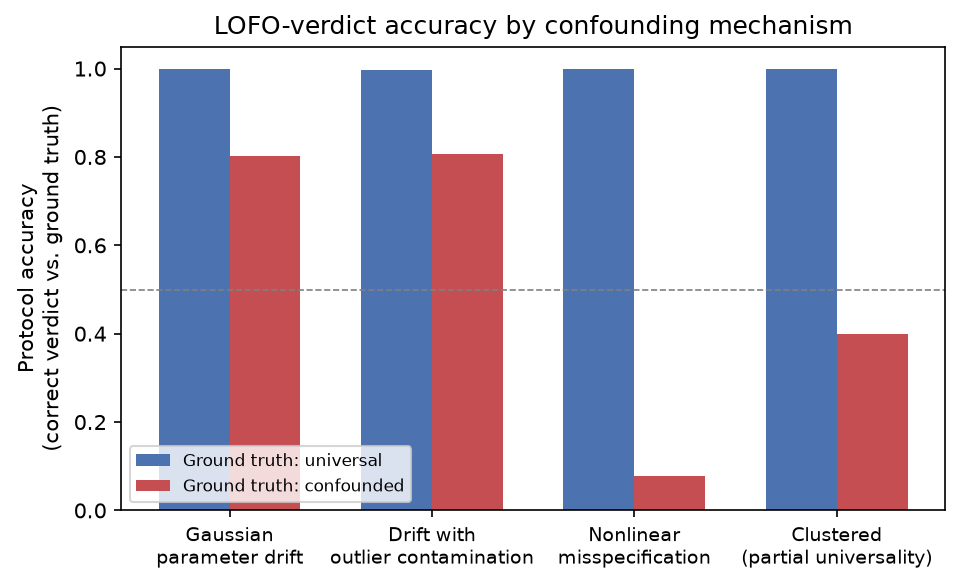
\includegraphics[width=0.85\textwidth]{figures/fig1_accuracy_by_confound_type.png}
\caption{LOFO-verdict accuracy by confounding mechanism, ground truth, and declaration rule (all four combinations reported in Table~\ref{tab:by-type}). The threshold rule (blue/red) is reliable against parameter drift and noise but has severe blind spots against nonlinear misspecification and clustered/partial universality; the permutation rule (purple/green) recovers most of the loss on exactly those two mechanisms, at the cost of a lower accuracy on truly universal data (purple, $\sim$94--95\% vs.\ the threshold rule's blue bars)}
\label{fig:accuracy-by-type}
\end{figure}

Unequal facility sizes (matching the real dataset's dispersion) have a comparatively minor effect on threshold-rule accuracy: 75.4\% pooled across mechanisms with equal facility sizes versus 76.7\% with unequal sizes.

\subsection{Meta-model: predicting verdict reliability from observable information}

This meta-model predicts the \emph{threshold rule's} own verdict correctness, not the permutation rule's (Sections~\ref{sec:results-v1}--\ref{sec:perm-vs-threshold} already show the permutation rule is preferable in absolute terms; this model quantifies how much a threshold-rule verdict specifically should be trusted, e.g.\ for readers of the companion manuscripts, which used the threshold rule). Because the target \texttt{correct} is itself imbalanced (the threshold rule is right 90.1\% and 76.1\% of the time overall on the first and second pass respectively, Sections~\ref{sec:results-v1}--\ref{sec:results-v2}), we report accuracy against a same-target majority-class baseline (always predicting the more common value of \texttt{correct}) rather than against 50\% or against the unrelated ground-truth-label base rate, correcting an omission in an earlier draft.

The gradient-boosting meta-model, trained on fully observable inputs (see Method), achieves 96.6\% test accuracy (AUC 0.952) on the first pass against a 90.1\% same-target baseline, predicting LOFO-verdict correctness from $K$, $n$, \texttt{obs\_sigma\_hat}, \texttt{obs\_hetero\_hat}, and the protocol's own observed output; a Gaussian process cross-check reaches 95.9\% accuracy (AUC 0.825, lower than the GBM's, indicating less well-calibrated probability estimates despite similar hard-label accuracy). On the second pass, the same observable-only feature set (plus \texttt{n\_mode\_unequal}) reaches a lower 85.5\% (AUC 0.893) against a 76.8\% baseline --- a modest but real +8.7-point gain, smaller than the raw accuracy figure alone would suggest; per-mechanism accuracy ranges from 77.4\% (nonlinear-misspecified) to 97.0\% (Gaussian drift). A separate \emph{oracle} variant, additionally given the confounding mechanism as an input a real practitioner would not know with certainty, reaches 91.8\% (AUC 0.935, +15.0 points over baseline); we report it as a what-if upper bound on how much knowing the mechanism could help, not as an observable-only result. Permutation importance for the observable-only model (Figure~\ref{fig:importance}) shows the protocol's own observed verdict and \texttt{obs\_sigma\_hat} jointly dominate; \texttt{obs\_hetero\_hat} contributes moderately, raw sample size ($K$, $n$) comparatively little.

\begin{figure}[tbp]
\centering
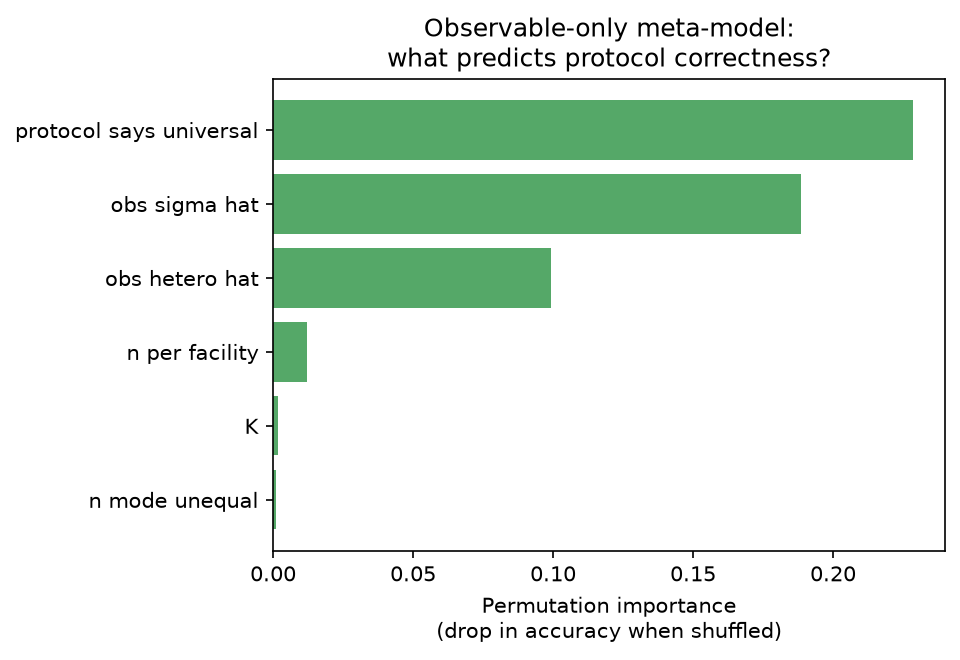
\includegraphics[width=0.85\textwidth]{figures/fig2_permutation_importance.png}
\caption{Permutation importance of design parameters and the protocol's own observed verdict, for predicting LOFO-verdict correctness}
\label{fig:importance}
\end{figure}

\subsection{Sample size within the ambiguous regime}
\label{sec:k-hard}

Restricting to the heterogeneity band where ground truth is genuinely hard to distinguish (Gaussian-drift mechanism, $h\in[0.5,1.5]$, $n{=}1355$ scenarios: 666 confounded, 689 universal), the universal arm is at ceiling for every $K$ bin by construction (100.0\% throughout under both rules, not tabulated separately) and the pooled figure used in an earlier version of this analysis mixed that ceiling in with the genuinely informative confounded-arm trend, diluting it. Restricted to the confounded arm only, the threshold rule shows no ``more facilities is better'' pattern -- if anything the opposite: 88.3\% at $K{=}2$--$3$, peaking at 96.2\% for $K{=}4$--$6$, then declining to 77.1\% by $K{=}16$--$20$ (Table~\ref{tab:k-hard}, Figure~\ref{fig:k-hard}). The permutation rule, on the same confounded-arm scenarios, is essentially unaffected by this decline: 93.3\% at $K{=}2$--$3$ and \emph{exactly} 100.0\% (106/106, 102/102, 103/103, 107/107, 188/188) for every larger $K$ bin tested. As in Section~\ref{sec:perm-vs-threshold}, more facilities does not rescue the threshold rule within this ambiguous regime, but it does not need to rescue the permutation rule, which is already reliable there.

\begin{table}[tbp]
\centering
\caption{LOFO-verdict accuracy vs.\ number of facilities $K$, ambiguous heterogeneity band ($h\in[0.5,1.5]$), Gaussian-drift mechanism, confounded arm only}
\label{tab:k-hard}
\small
\begin{tabular}{lccc}
\toprule
$K$ bin & $n$ & Threshold rule & Permutation rule \\
\midrule
2--3   & 60  & 0.883 & 0.933 \\
4--6   & 106 & 0.962 & 1.000 \\
7--9   & 102 & 0.853 & 1.000 \\
10--12 & 103 & 0.893 & 1.000 \\
13--15 & 107 & 0.841 & 1.000 \\
16--20 & 188 & 0.771 & 1.000 \\
\bottomrule
\end{tabular}
\end{table}

\begin{figure}[tbp]
\centering
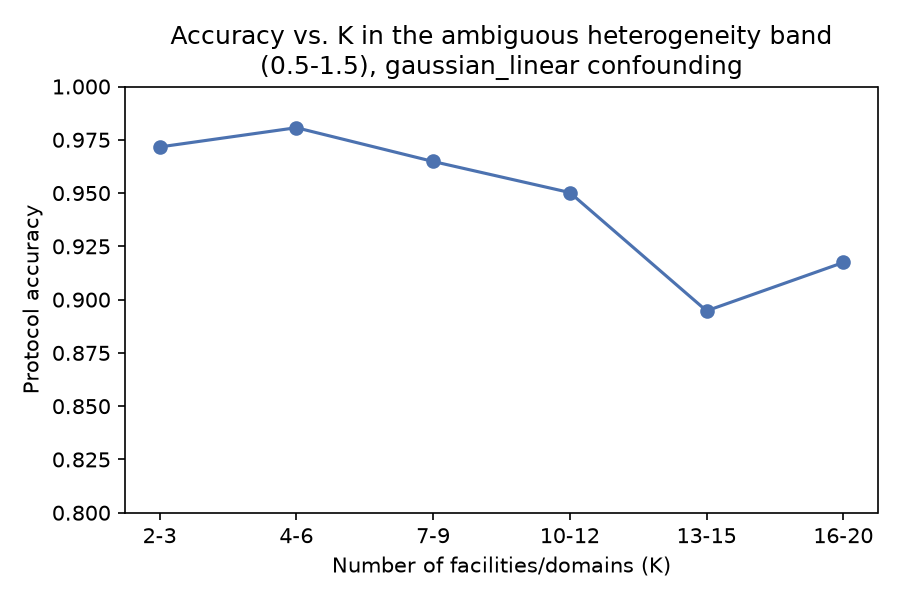
\includegraphics[width=0.7\textwidth]{figures/fig3_accuracy_vs_K_hard_band.png}
\caption{LOFO-verdict accuracy versus number of facilities $K$, restricted to the ambiguous heterogeneity band and the confounded arm only, Gaussian-drift mechanism: threshold rule vs.\ permutation rule}
\label{fig:k-hard}
\end{figure}

\subsection{Covariate-support overlap decides which rule is valid (third pass)}
\label{sec:results-v3}

The permutation rule's advantage in Sections~\ref{sec:results-v1}--\ref{sec:results-v2} was established on scenarios where all facilities share complete covariate support. Table~\ref{tab:overlap} and Figure~\ref{fig:overlap} report the third pass (6,000 scenarios, overlap sampled uniformly), scoring all three declaration rules on the universal arm (where any rejection is a false alarm) and the confounded arm (where any rejection is a correct detection).

The naive permutation test is calibrated only at the high-overlap end. Its false-alarm rate rises monotonically as the facilities' operating windows separate, from 5.9\% at overlap 0.8--1.0 --- essentially the nominal $\alpha=0.05$, and the regime both earlier passes occupy --- to 17.2\% at overlap 0.0--0.2, roughly \emph{threefold} anti-conservative. The mechanism is the one anticipated in the Method: with separated windows, predicting a held-out facility is extrapolation, while the permuted pseudo-folds remain interpolation, so a universal law still looks anomalously bad relative to its own permutation null. The threshold rule is immune to this by construction, never producing a false alarm at any overlap level, which is precisely the property that makes it a safe fallback.

Stratifying the permutation repairs the problem essentially for free. Restricting label swaps to within-stratum swaps holds the false-alarm rate at 4.6--6.2\% across the entire overlap range while keeping power at 97.7\% or above --- against the threshold rule's 82.6--89.5\%. On these scenarios the stratified test therefore dominates both alternatives, and it is the rule we recommend.

\paragraph{The identifiability limit.} That dominance has a boundary. In the extreme corner (overlap $<0.02$, $n{=}101$ scenarios) the stratified test's own power falls to 77.8\% and its false-alarm rate rises to 8.9\%. At \emph{exactly} disjoint windows it degenerates completely: in a dedicated batch of 150 scenarios per arm at overlap $=0$ (\texttt{degenerate\_corner\_overlap\_zero} in \texttt{results/synth\_scenarios\_v3\_summary.json}) the stratified test returns a 0.0\% false-alarm rate and 0.0\% power --- with facility identity a deterministic function of the covariates, each stratum contains a single facility, no label swap is admissible, and the test cannot reject anything. The naive test in that same corner reaches a 20.0\% false-alarm rate, while the threshold rule holds 0.0\% false alarms at 85.3\% power. This is not a defect of the estimator but an identifiability limit --- under perfect separation, ``the facilities follow different laws'' and ``the facilities were run at different conditions'' are not distinguishable by any argument based on permuting facility labels. Where a corpus approaches that corner, the plain threshold rule is the defensible choice, accepting roughly 16 points of power to retain a zero false-alarm rate.

\begin{table}[tbp]
\centering
\caption{False-alarm rate (universal arm) and power (confounded arm) by covariate-support overlap between facilities, third pass. Nominal significance level $\alpha=0.05$ for both permutation rules}
\label{tab:overlap}
\small
\begin{tabular}{lcccc|ccc}
\toprule
 & & \multicolumn{3}{c|}{False-alarm rate} & \multicolumn{3}{c}{Power} \\
Overlap & $n_{\text{univ}}$ / $n_{\text{conf}}$ & Thr. & Perm. & Perm.-strat & Thr. & Perm. & Perm.-strat \\
\midrule
0.0--0.2 & 574 / 604 & 0.000 & 0.172 & 0.056 & 0.826 & 1.000 & 0.978 \\
0.2--0.4 & 582 / 624 & 0.000 & 0.125 & 0.062 & 0.840 & 1.000 & 1.000 \\
0.4--0.6 & 564 / 596 & 0.000 & 0.105 & 0.053 & 0.874 & 1.000 & 1.000 \\
0.6--0.8 & 613 / 621 & 0.000 & 0.070 & 0.052 & 0.895 & 1.000 & 1.000 \\
0.8--1.0 & 591 / 631 & 0.000 & 0.059 & 0.056 & 0.870 & 0.998 & 1.000 \\
\bottomrule
\end{tabular}
\end{table}

\begin{figure}[tbp]
\centering
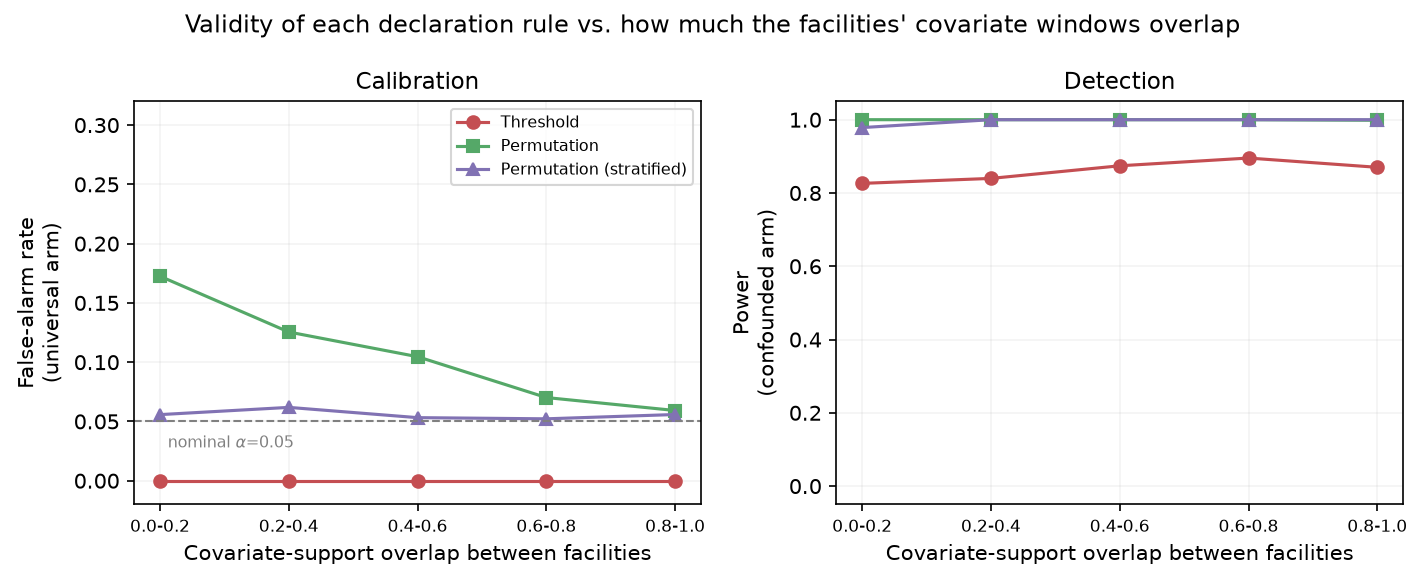
\includegraphics[width=0.98\textwidth]{figures/fig4_overlap_calibration_power.png}
\caption{Validity of each declaration rule against covariate-support overlap. Left: false-alarm rate on truly universal scenarios, against the nominal $\alpha=0.05$. Right: power on truly confounded scenarios. The naive permutation rule loses calibration as facilities separate; the stratified variant holds calibration and power across the range; the threshold rule never false-alarms but detects least}
\label{fig:overlap}
\end{figure}

\paragraph{Where the companion corpus falls.} Because the choice of rule depends on a quantity that can be measured, we computed the same statistic on the companion manuscripts' 114-point windage corpus (a description of its design, not a re-analysis of its windage relationship; \texttt{results/companion\_overlap.json}). Its four facilities have a mean pairwise support overlap of 0.32 in $\log Re$, but that mean hides the structure that matters: the three smaller facilities overlap substantially with each other (0.53--0.69), while the largest, contributing 45 of the 114 points, is essentially disjoint from all three (0.009, 0.000, 0.000). A naive permutation test applied to that corpus would therefore run at roughly 2.5 times its nominal false-alarm rate, and the fold holding out its largest facility sits in the degenerate corner described above. This does not disturb the companion studies' own conclusion, which was reached with the threshold rule --- the one rule that never false-alarms at any overlap in our sweep. It does mean that the naive permutation test, despite being the better rule on the first two passes, would have been the wrong tool for that particular dataset, and that the stratified variant is the appropriate one there.

\subsection{External check: the real windage case's observed verdict}
\label{sec:anchor}

Evaluated at the real windage case's design point ($K{=}4$, $n\approx28.5$) using its \emph{observed} LOFO verdict (\texttt{protocol\_says\_universal}=\textsc{False}, from the second companion manuscript's reported pooled LOFO R\textsuperscript{2}=$-0.885$ \citep{gilruiz2026paper2}) and a 25-point grid over plausible \texttt{obs\_sigma\_hat}$\in[0.1,0.5]$ and \texttt{obs\_hetero\_hat}$\in[0.1,1.2]$, the gradient-boosting meta-model estimates the verdict is correct with probability 0.997--0.999 (mean 0.999) across the entire grid; the Gaussian process cross-check gives a markedly lower, equally stable 0.627--0.633 (mean 0.630).

\paragraph{The GBM's near-certainty here is a property of the generator, not case-specific evidence.} We checked this directly rather than take the flat 0.997--0.999 sweep at face value. Across all 1,590 first-pass scenarios sharing the real case's observed verdict (\texttt{protocol\_says\_universal}=\textsc{False}), regardless of $K$, $n$, or the observable proxies, \texttt{correct}=1 exactly 1.0000 of the time (1,590/1,590, \texttt{results/meta\_model\_results.json}). The reason is structural. By construction, the universal arm of this generator has no facility-to-facility deviation to produce a spurious LOFO$<0$ result, so a genuinely universal scenario essentially never yields \texttt{protocol\_says\_universal}=\textsc{False} in the first place; conditioning on that observed verdict already near-determines the ground truth is confounded, independent of anything else about the scenario. The GBM has correctly learned this regularity of the synthetic generator. It has not learned anything about the real windage case specifically, and the flat, featureless sweep in the previous paragraph is a symptom of exactly that: if the GBM's probability depended meaningfully on $K$/$n$/the observable proxies, the sweep would vary. It does not, because the decisive feature is only ever \texttt{protocol\_says\_universal}, which is fixed at \textsc{False} for the whole sweep. The GP cross-check's lower, noisier estimate is arguably the more honest of the two numbers here: its RBF kernel cannot represent the near-deterministic relationship as cleanly, so it partially regresses toward the surrounding class balance instead of memorizing this generator-specific regularity.

The check still has some value, just far less than a 99.7--99.9\% figure suggests: it shows that this generator design essentially never produces a false ``not universal'' verdict on truly universal data, so, taking the companion study's LOFO$<0$ result at face value, false-alarm-driven non-generalization is an unlikely explanation \emph{under the mechanisms this generator represents}. What it does \emph{not} show is that the real case's own confounding is of a kind this protocol reliably detects: Table~\ref{tab:by-type} shows the threshold rule used in the companion study detects confounding only 9.4\% of the time when it is of the nonlinear-misspecification type and 42.7\% when clustered, and this anchor computation cannot distinguish which mechanism, if any, applies to the real windage data (its true \texttt{obs\_sigma\_hat}/\texttt{obs\_hetero\_hat} are not computed here, deliberately, to avoid re-analyzing the companion manuscript's raw data). We therefore downgrade this check, relative to an earlier draft, from ``support for the companion finding'' to: a demonstration that the specific failure mode of a false-positive confounding call is implausible under this generator, alongside an explicit acknowledgment that it cannot rule out the harder-to-detect mechanisms this same paper identifies. A reader wanting a genuine external check specific to the real case's own confounding mechanism would need the raw-data re-analysis this paper's scope deliberately excludes.

\section{Discussion}

The single most actionable recommendation from this study is a two-step procedure rather than a single rule. \emph{First, measure how much your data sources actually overlap in covariate space}; the statistic is the mean pairwise intersection-over-union of their covariate ranges (Method), it needs nothing but the design matrix, and it decides which of the following applies. \emph{Second, choose the declaration rule accordingly}:

\begin{itemize}
  \item \textbf{Overlap above $\sim$0.05, the common case}: use the \emph{stratified} facility-label permutation test. It is computed from the same fits a LOFO audit already produces, requires no additional data collection, closes most of the gap between the threshold rule's best mechanism (Gaussian drift, 82.3\% detection) and its worst (nonlinear misspecification, 9.4\% detection), and unlike the naive permutation test it stays calibrated as the sources separate (Table~\ref{tab:overlap}).
  \item \textbf{Overlap near zero}: use the plain LOFO$>0$ threshold. It detects less (roughly 16 points less power), but it is the only rule in our sweep that never produces a false alarm, and in this regime no permutation-based alternative is trustworthy.
\end{itemize}

The naive permutation test, which the first two passes alone would have recommended without qualification, is the rule we would now advise against as a default: it is the strongest option when supports overlap and the weakest when they do not, and which of those a practitioner is in is not visible from the LOFO output itself. That the earlier passes could not see this is instructive in its own right --- a benchmark that samples only one corner of the design space will confidently recommend a method that fails outside it.

Where a LOFO+bootstrap audit has already been run with the plain threshold, as in the companion manuscripts, this study's role is instead diagnostic: knowing which regime the threshold rule is in changes how much its verdict should be trusted.

A secondary implication runs against the intuitive fix of ``collect more facilities.'' Within the tested range, raw facility count is a weak predictor of the threshold rule's reliability once the type and strength of confounding are accounted for, and for nonlinear misspecification specifically, more facilities make the threshold rule \emph{worse}, not better (Section~\ref{sec:results-v2}). The practical guidance this study supports is: \emph{know, or test for, the shape of the suspected confounding before trusting a threshold-rule LOFO verdict --- or use a permutation rule, which does not require knowing it, having first checked that the sources overlap enough for one to be valid.} A threshold-rule audit that declares ``universal'' should not be read as ruling out facility-specific structure if that structure could plausibly be nonlinear or clustered --- the threshold rule is nearly blind to both, though the permutation rules are not (Table~\ref{tab:by-type}). What does help, and is worth designing for in advance, is arranging that the sources share operating conditions: overlap is what buys access to the more powerful rules (Table~\ref{tab:overlap}), and it is a property of how a corpus is assembled rather than of how many facilities it contains. This has an implication for the second companion manuscript \citep{gilruiz2026paper2}, which used the threshold rule: its finding of \emph{non-generalization} is consistent with the regime where the threshold rule is reliable, and Section~\ref{sec:anchor} shows this generator design rarely produces a false ``not universal'' call on truly universal data, but confirming this more specifically for the real windage case's own confounding mechanism would need the \emph{stratified} permutation rule --- the appropriate one at that corpus's measured overlap (Section~\ref{sec:results-v3}) --- applied directly to that dataset, which is the raw-data re-analysis this paper's scope excludes. Any future work in this series reporting a \emph{positive} generalization result from the threshold rule alone should be treated cautiously unless nonlinear and clustered alternatives have been separately ruled out, ideally by also checking the permutation-rule verdict.

\section{Limitations}

The synthetic generator uses a single base functional form (two-predictor log-linear power law) matching the second companion manuscript's winning model \citep{gilruiz2026paper2}; other functional forms, higher-dimensional predictor sets, or non-log-linear ground truths are not explored. Each scenario is a single random draw, not repeated across seeds, so scenario-level accuracy estimates carry sampling noise not fully reflected in the reported point estimates (binomial 95\% confidence intervals are reported in Table~\ref{tab:by-type} for the headline per-mechanism figures; individual cells in finer breakdowns, e.g. $K$ bins in Figure~\ref{fig:k-hard}, are noisier still and not individually interval-estimated). The real-case anchor sweeps both observable proxies over a plausible range rather than computing their true values for the real case, deliberately to avoid re-analyzing the companion manuscript's raw data; this means the anchor is illustrative sensitivity analysis, not a precise recovery, and the two meta-models it uses disagree with each other by a wide margin (Section~\ref{sec:anchor}), which should temper how much weight is placed on it.

The meta-model's feature set excludes three quantities a reader should know were once included by mistake: the scenario's ground-truth label (which trivially determines the correctness target), the generator's latent noise/heterogeneity settings (not computable from real data despite an earlier claim otherwise), and, in the current oracle variant only, the confounding mechanism (kept, but reported separately from the observable-only result rather than pooled with it). All three are recorded here because they affect how the reported accuracy numbers should be read, not as narrative detail.

A bug in the clustered-mechanism generator, fixed before the results reported here, could, with probability $\approx1/2^{K-1}$ per scenario, assign every facility to the same latent cluster, silently mislabeling a handful of nominally ``confounded'' clustered scenarios as truly universal ($\approx$5\% of draws at small $K$). All second-pass numbers in this manuscript were generated after this fix (rejection sampling requiring at least two distinct clusters); we flag it because a reader comparing against an earlier internal draft's numbers would otherwise see an unexplained shift in the clustered-mechanism figures.

The four confounding mechanisms are not calibrated to a common effect size: the heterogeneity parameter $h$ enters the intercept, the linear slopes, and the nonlinear-misspecification quadratic term with different fixed multipliers, so at equal $h$ the mechanisms do not necessarily perturb the fitted model by an equal amount. Part of the reported ordering of mechanisms by threshold-rule detection difficulty (Table~\ref{tab:by-type}) may therefore partly reflect this generator design choice rather than a mechanism-intrinsic property; we did not attempt to re-calibrate the mechanisms to a common effect-size scale, and flag the ordering across mechanisms as correspondingly less certain than the within-mechanism findings (e.g.\ the permutation-vs-threshold comparison, Table~\ref{tab:by-type}, which compares two rules on the identical scenarios and is not affected by this issue). Relatedly, and left entirely to future work: we conjecture, without deriving or independently verifying it here, that the threshold rule's detection power for nonlinear misspecification may be structurally near-zero rather than merely low when the facility-specific nonlinear term is close to orthogonal to the fitted model's column space -- consistent with, but a stronger claim than, the empirical power curves in Section~\ref{sec:results-v2}.

The overlap analysis has boundaries of its own. It separates facilities along a single covariate ($\log Re$, the axis on which the companion corpus actually separates); real designs can differ along several covariates at once, or in ways that are not simple window shifts, and we have not characterized how the two permutation rules behave under those richer forms of design separation. The stratified variant uses $K$ equal-count strata throughout, a defensible default but not a tuned choice: the number of strata trades control of design confounding against the number of admissible label swaps, and we did not attempt to optimize it. The third pass also uses only the Gaussian-drift confounding mechanism, so the overlap effect is characterized cleanly but is not crossed with the other three mechanisms, and the overlap threshold of $\approx$0.05 below which we advise falling back to the threshold rule is read off Table~\ref{tab:overlap} rather than derived. Finally, the third pass fixes facility sizes as equal and omits the bootstrap diagnostic, both of which are characterized in the earlier passes but not re-crossed with overlap here.

\section{Conclusion}

We show, via a three-pass synthetic study with both LOFO cross-validation and facility-level bootstrap implemented, that under the conventional LOFO$>0$ threshold rule, a standard cross-domain audit protocol for scaling-law discovery is reliable against simple parameter drift and heavy noise but has severe, quantified blind spots against nonlinear model misspecification and clustered (partial) universality that do not shrink, and for nonlinear misspecification worsen, with more facilities. A facility-label permutation test, computed from the same fits at no extra data-collection cost, closes most of this gap. Its validity is not unconditional, however, and the condition is one earlier passes could not see: the permutation null requires the facilities to share covariate support, and the naive test becomes up to threefold anti-conservative as their operating windows separate. Permuting labels only within covariate strata restores calibration across the range at essentially no cost in power, and is the rule we recommend, with the plain threshold rule -- the only rule that never false-alarms -- as the fallback under near-total separation, where no label-permutation argument can distinguish a different law from a different design. Since the appropriate rule depends on a statistic practitioners can compute from their own design matrix, we define it, report it for the companion corpus, and give the resulting decision rule. An observable-only meta-model estimator, applied to the real windage case's own observed threshold-rule verdict \citep{gilruiz2026paper1,gilruiz2026paper2}, gives near-certain but largely tautological support (0.627--0.999 across its two implementations, the higher number reflecting a structural property of the generator rather than case-specific evidence, as we verify directly) to the narrower claim that a false-positive confounding call is an unlikely explanation for that verdict -- an illustrative check, not independent confirmation that the real case's own confounding mechanism is one this protocol reliably detects. This closes the three-manuscript arc --- audit protocol, real-world application, and a characterization of the protocol's own reliability boundaries, including a fix for its main blind spot and an explicit account of when that fix itself applies --- with a result directly actionable for anyone applying this class of method to a domain with a broadly similar confounding structure.

\begin{appendix}
\section{Minimum Verifiable Facts from the Companion Manuscripts}
\label{app:companion}

This paper's motivation, and its external check in Section~\ref{sec:anchor}, depend on numbers reported in two unpublished companion manuscripts \citep{gilruiz2026paper1,gilruiz2026paper2} that a reader of this paper alone cannot independently inspect. To limit how much of the argument rests purely on our own say-so, we restate here the small set of facts those sections actually depend on, without adding any number not already used in the main text:

\begin{itemize}
  \item The real windage dataset has $N=114$ points across four facilities, with reported sizes 45, 41, 20, and 8.
  \item The companion study's winning pooled model (log-linear, four Buckingham-$\Pi$ predictors) reaches in-sample R\textsuperscript{2}$=0.870$ but pooled leave-one-facility-out R\textsuperscript{2}$=-0.885$ in log space.
  \item Of that model's coefficients, only the Reynolds-number exponent's bootstrap confidence interval excludes zero; the companion manuscript reports this as the sole coefficient that survives facility-level bootstrap resampling.
  \item The four facilities' $\log_{10} Re$ windows are $[6.80, 7.91]$, $[5.47, 6.82]$, $[4.96, 6.72]$ and $[5.57, 6.51]$, giving pairwise support overlaps of 0.009, 0.000 and 0.000 between the largest facility and each of the other three, and 0.530--0.691 among those three, for a mean pairwise overlap of 0.317 (Section~\ref{sec:results-v3}).
\end{itemize}

The fourth item is a statement about where each facility sits in Reynolds space --- a property of the corpus's design, readable in principle from the four original published sources --- and not an estimate of the windage relationship, so reporting it does not breach the scope limit below. It is included because Section~\ref{sec:results-v3} shows the choice of declaration rule depends on it, and a reader cannot check that choice without it.

We do not restate, and did not re-derive, any finer-grained breakdown (e.g.\ per-facility fitted coefficients or $C_p$ values) from the companion manuscripts' raw data, since doing so would constitute the re-analysis this paper's scope deliberately excludes (Introduction). A reader who needs to audit these three facts directly should request the companion manuscripts or their eventual published versions from the corresponding author.
\end{appendix}

\begin{Backmatter}

\paragraph{Acknowledgments}
Large language model assistance (Claude Sonnet 5 and Claude Opus 5, Anthropic, August 2026) was used for code implementation, literature search and reference verification, synthetic-experiment design, and manuscript drafting. All code was executed and its output inspected by the corresponding author; the corresponding author checked available DOI or publisher metadata for each cited reference that has one (the two unpublished companion manuscripts were checked against their own source files instead, since neither has a public record yet).

\paragraph{Funding Statement}
No external funding.

\paragraph{Competing Interests}
The authors declare no competing interests.

\paragraph{Data Availability Statement}
All synthetic scenario generation, audit protocol, and meta-model code, together with all reported summary statistics, are publicly available at \url{https://github.com/jesusgilru-prog/audit-protocol-reliability-dce}, tagged release \texttt{v2.0-overlap} for a stable, citable snapshot matching the numbers reported in this manuscript. Generated with fixed random seeds for exact reproducibility, hardcoded as \texttt{RNG\_SEED} at the top of each generation script and reported in the corresponding summary JSON files (\texttt{20260818} for the first and second passes and the meta-models, \texttt{20260825} for the third). A permanent Zenodo DOI archiving this repository will be minted and added here upon acceptance.

\paragraph{Ethical Standards}
This study uses only synthetic data and summary statistics reported in companion manuscripts by the corresponding author; it involves no human or animal subjects and no new experimental data collection.

\paragraph{Author Contributions}
Conceptualization: J.G.R. Methodology: J.G.R. Software: J.G.R. Data curation: J.G.R. Writing original draft: J.G.R. Validation: R.A.P.D., C.E.M.M. Writing -- review and editing: R.A.P.D., C.E.M.M.

\bibliographystyle{plain}
\bibliography{refs}

\end{Backmatter}

\end{document}
